\begin{problem}[Practice Exam 1, Problem 1]
    Let \( X = (X_n)_{n\in\NN_0} \) be a discrete time Markov chain with \( X_n \) representig the amount of water in a reservoir at noon on day \( n \). Assume \( X_0 \in \NN_0 \). Let \( Y = (Y_n)_{n\in\NN_0} \) be a sequence of iid random variables with \( Y_n \) representing the aount of water that flows into the reservoir during the \( n \)-th day. The state space of \( Y \) is \( \{0,1,2,\ldots \} \). The resevoir has a maximum capacity of \( K\in\NN \). When the resevoir is filled to level \( K \), all excssive inflows are lost.
    \begin{enumerate}[nolistsep,label=(\alph*)]
        \item Write the one-step transition matrix \( P \) of \( X \) in terms of the probability generating function \( G_Y \) of \( Y \).
        \item Find an expression for the stationary distribution \( \pi \) of \( X \) in terms of the probability generating function \( G_Y \) of \( Y \).
    \end{enumerate}
\end{problem}

\begin{solution}[Solution]
\begin{enumerate}[label=(\alph*)]
    \item 
        We assume all the water comes in the afternoon. That is, \( X_{n+1} = X_n + Y_n \).

        Suppose on day \( n \) the resevoir is not full. That is, \( X_n = k < K \). If it is not filled completely by the incoming water, then some amount of water \( j < K-k \) was added. In this case \( X_{n+1} = k+j \) with probability,
        \begin{align*}
            \PP(Y_n = j) = f_Y(j) = 
            \left[\frac{1}{j!}\dd[j]{G_Y(s)}{s} \right]_{s=0}
        \end{align*}
        
        Otherwise, \( X_{n+1} = K \) with probability,
        \begin{align*}
            1-\sum_{j < K-k} f_Y(j) = 1 - \sum_{j<K-k} \left[\frac{1}{j!} \dd[j]{G_Y(s)}{s} \right]_{s=0}
        \end{align*}
        
        Suppose \( X_n = K \). Then since no water leaves the resevoir, \( X_{n+1} = K \) with probability one.

        We can write this as,
        \begin{align*}
            X_{n+1} = \begin{cases}
                0 & j < i \\
                \left[\frac{1}{j!}\dd[j]{G_Y(s)}{s} \right]_{s=0} & j < K - X_n \\ \\
                1 - \sum_{j<K-X_n} \left[\frac{1}{j!}\dd[j]{G_Y(s)}{s} \right]_{s=0} & \text{otherwise}
            \end{cases}
        \end{align*}
       
        Conditioning on \( X_n = i \) we then have,
        \begin{align*}
            P_{i,j} = \PP(X_{n+1} = j | X_n = i) = 
             \begin{cases}
                0 & j < i \\
                \left[\frac{1}{j!}\dd[j]{G_Y(s)}{s} \right]_{s=0} & j < K - i \\ \\
                1 - \sum_{j<i} \left[\frac{1}{j!}\dd[j]{G_Y(s)}{s} \right]_{s=0} & \text{otherwise}
            \end{cases}
        \end{align*}


    \item
        Note that \( \pi = [0,0,\ldots,0,1] \) is a stationary distribution.

        \note{argue the distributoin is unique?}


        \note{alternative approach??}
        Clearly \( X_n \to K \) as \( n\to\infty \).

        \note{in what sense?}
        
\end{enumerate}
\end{solution}

\begin{problem}[Practice Exam 1, Problem 2]
    Let \( (X,Y) = (X_t,Y_t)_{t\geq 0} \) satisfy the following SDE,
    \begin{align*}
        \d X_t = \d W_t^1, && \d Y_t = \d W_t^2, && (X_0,Y_0) = (x,y)
    \end{align*}
    where \( W = (W_t^1,W_t^2)_{t\geq 0} \) is a two-dimensinoal Brownian motion with independent components. Define a process \( (R,\Phi) = (R_t,\Phi_t)_{t\geq 0} \) as follows,
    \begin{align*}
        \Phi_t = \arctan(Y_t/X_t), && R_t^2 = X_t^2 + Y_t^2
    \end{align*}
    \begin{enumerate}[nolistsep,label=(\alph*)]
        \item Derive the SDEs satisfied by \( (R,\Phi) \).
        \item Define,
            {\small
            \begin{align*}
                u(r,\phi) = \EE \left[ e^{-\lambda \tau} f(R_\tau) | R_0 = r,\Phi_0 = \phi \right], &&
                \tau = \inf\{t\geq 0:\Phi_t\notin(0,\pi/2)\}, &&
                \phi \in (0,\pi/2)
            \end{align*}
            }
            Derive a PDE satisfied by \( u \).
        \item Desribe with pseudo-code how you would find \( u(r,\phi) \) using Monte Carlo simulation.
    \end{enumerate}    
\end{problem}

\begin{solution}[Solution]
\begin{enumerate}[label=(\alph*)]
    \item Define \( f(x,y) = \arctan(y/x) \) and \( g(x,y) = \sqrt{x^2+y^2} \). Now note that,
        \begin{align*}
            \Phi_t = f(X_t,Y_t), && R_t = g(X_t,Y_t)
        \end{align*}

        Appying It\^o's formula we find,
        \begin{align*}
            \d \Phi_t &=  f_x(X_t,Y_t)\d X_t + f_y(X_t,Y_t)\d Y_t 
            \\&\hspace{3em}+ \frac{1}{2}\big(f_{xx}(X_t,Y_t)\d[X,X]_t + f_{xy}(X_t,Y_t)\d [X,Y]_t 
            \\&\hspace{6em}+ f_{yx}(X_t,Y_t)\d[Y,X]_t + f_{yy}(X_t,Y_t)\d[Y,Y]_t\big) 
        \end{align*}
        
        Using our Heuristics we have,
        \begin{align*}
            \d[X,X]_t = \d[Y,Y]_t = \d t, && \d[X,Y]_T = \d[Y,X]_t = 0
        \end{align*}
        
        We compute,
        \begin{align*}
            f_x(x,y) &= -\frac{y}{x^2+y^2} = - \frac{\sin(\arctan(y/x)}{\sqrt{x^2+y^2}} \\
            f_y(x,y) &= \frac{x}{x^2+y^2} = \frac{\cos(\arctan(y/x))}{\sqrt{x^2+y^2}}\\
            f_{xx}(x,y) &= \frac{2xy}{(x^2+y^2)^2} \\ 
            f_{yy}(x,y) &= -\frac{2xy}{(x^2+y^2)^2}
        \end{align*}
        
        Therefore, maxing the substitutions, \( \Phi_t = \arctan(Y_t/X_t) \), and \( R_t = \sqrt{X_t^2+Y_t^2}  \),
        \begin{align*}
            \d \Phi_t &= - \frac{\sin(\Phi_t)}{R_t}\d W_t^1 + \frac{\cos(\Phi_t)}{R_t}\d W_t^2
        \end{align*}
        
        Similarly,
        \begin{align*}
            \d R_t &=  g_x(X_t,Y_t)\d X_t + g_y(X_t,Y_t)\d Y_t
            \\&\hspace{3em}+ \frac{1}{2}\big(g_{xx}(X_t,Y_t)\d[X,X]_t + g_{xy}(X_t,Y_t)\d [X,Y]_t 
            \\&\hspace{6em}+ g_{yx}(X_t,Y_t)\d[Y,X]_t + g_{yy}(X_t,Y_t)\d[Y,Y]_t\big) 
        \end{align*}
        
        We compute,
        \begin{align*}
            g_x(x,t) &= \frac{x}{\sqrt{x^2+y^2}} = \cos(\arctan(y/x)) \\
            g_y(x,t) &= \frac{y}{\sqrt{x^2+y^2}} = \sin(\arctan(y/x)) \\
            g_{xx}(x,t) &= \frac{y^2}{(x^2+y^2)^{3/2}} \\
            g_{yy}(x,t) &= \frac{x^2}{(x^2+y^2)^{3/2}}
        \end{align*}
        
        Therefore, maxing the substitutions, \( \Phi_t = \arctan(Y_t/X_t) \), and \( R_t = \sqrt{X_t^2+Y_t^2}  \),
        \begin{align*}
            \d R_t &= \cos(\Phi_t)\d W_t^1 + \sin(\Phi_t) \d W_t^2 + \frac{1}{2R_t} \d t
        \end{align*}


    \item
        We know \( u \) satisfies,
        \begin{align*}
            (\cA - \lambda) u = 0, && u(r,0) = u(r,\pi/2) = f(r)
        \end{align*}
        where,
        \begin{align*}
            \cA = \frac{1}{2r} \partial_r + \frac{1}{2}\left(\partial_r + \frac{1}{r^2}\partial_\phi^2 \right)
        \end{align*}
        

        \iffalse
        Define,
        \begin{align*}
            v(r,\phi) = \EE[e^{-\lambda(\tau - t)}f(R_\tau) | X_t=x, \Phi_t =\phi]
        \end{align*}
        
        Define,
        \begin{align*}
            M_t &= e^{-\lambda t} v(R_t,\Phi_t)
            \\&= e^{-\lambda t} \EE[e^{-\lambda (\tau - t)}f(R_\tau) | X_t = x, \Phi_t = \phi]
            \\&= \EE[e^{-\lambda \tau}f(R_\tau) | X_t = x, \Phi_t = \phi]
        \end{align*}
        

        We claim that \( M_t \) is a Martingale. Indeed,
        \begin{align*}
            \EE[ M_t | \cF_s] 
            &= \EE[\EE[ e^{-\lambda \tau} f(R_\tau) | R_t,\Phi_t] | \cF_s]
            \\&= \EE[\EE[ e^{-\lambda \tau} f(R_\tau) | \cF_t] | \cF_s]
            \\&= \EE[ e^{-\lambda \tau} f(R_\tau) | \cF_s]
            \\&= M_s
        \end{align*}
        
        Using our Heuristics \( \d W_t^1 \d W_t^1 = \d W_t^2 \d W_t^2 = \d t \) and \( \d W_t^1 \d W_t^2 = \d t\d W_t^1 = \d t \d W_t^2 = \d t \d t = 0 \) we compute,
        \begin{align*}
            \d[R,R]_t &= 0 \\ %&= \cos^2(\Phi_t) \d t + \sin^2(\Phi_t)\d t = \d t \\
            \d[R,\Phi]_t &=  - \frac{\sin(\Phi_t)\cos(\Phi_t)}{R_t}\d t + \frac{\cos(\Phi_t)\sin(\Phi_t)}{R_t}\d t = 0\\
            \d[\Phi,\Phi]_t &= \frac{\sin^2(\Phi_t)}{R_t^2}\d t + \frac{\cos(\Phi_t)^2}{R_t^2}\d t = \frac{1}{R_t^2}\d t
        \end{align*}
        

        Therefore,
        \begin{align*}
            \d M_t &= \d \left( e^{-\lambda t} v(R_t,\Phi_t) \right) \\
            &= \d \left( e^{-\lambda t} \right) v(R_t,\Phi_t) + e^{-\lambda t} \d v(R_t,\Phi_t)
        \end{align*}
        \fi

\iffalse
        Therefore,
        \begin{align*}
            \d u(R_t,\Phi_t) &= \partial_r u(R_t,\Phi_t) \d R_t + \partial_\phi u(R_t,\Phi_t) \d \Phi_t
            \\& \hspace{3em}+ \frac{1}{2} \big( \partial_r^2 u (R_t,\Phi_t) \d[R,R]_t + 2\partial_{r\phi} u(R_t,\Phi_t) \d[R,\Phi]_t 
            \\&\hspace{6em}+ \partial_{\phi}^2 u(R,\Phi)\d[\Phi,\Phi]_t \big)
            \\&= \left( \frac{1}{2R_t}\partial_r + \frac{1}{2} \frac{1}{R^2}\partial_\phi^2  \right)u(R_t,\Phi_t)\d t + (\cdots)\d W_t^1 + (\cdots)\d W_t^2
        \end{align*}
        
        Since \( u(R_t,\Phi_t) \) is a martingale, the \( \d t \) term must be zero. Therefore,
        \begin{align*}
            \left( \frac{1}{r} \partial_r + \frac{1}{r^2}\partial_\phi^2  \right) u(r,\phi) = 0
        \end{align*}
        
        We have boundary conditions,
        \begin{align*}
            u(r,0) = u(r,\pi/2) = f(r)
        \end{align*}
        \fi 


    \item We can compute \( u(r,\phi) \) by simulating trajectories of \( R \) and \( \Phi \), and observing where they end up. In particular, starting at the point \( (R_0,\Phi_0) = (r,\phi) \), we run a stochastic integrator (forward Euler for instance) until the process exits. We then compute the value of \( e^{-\lambda \tau} f(R_\tau) \). Repeating this integration many times will give an estimate at the expected value.

        To integrate we must set a time step size \( \Delta t \). At each step \( \d W_t^1 \) and \( \d W_t^2 \) will be normally distributed with mean 0 and variane \( \Delta t \). To advance the solution we generate random normal variables with this mean and variance, and then compute the change using our SDEs for \( R \) and \( \Phi \), replacing \( \d t \) with \( \Delta t \) and \( \d W_t^1, \d W_t^2 \) with the random normal variables. This is repeated iteratively.

\end{enumerate}
\end{solution}


\begin{problem}[Practice Exam 2, Problem 1]
Let \( Y = (Y_n)_{n\in\NN_0} \) be a sequence of iid random variables with \( Y_n\sim \operatorname{Pois}(\lambda) \) representing the number of particles entering a chamer at time \( n \). The lifetimes of the particles are iid geometric random variables with parameter \( p \). Let \( X_n \) represent the number of particles in the chamber at time \( n \).
\begin{enumerate}[nolistsep,label=(\alph*)]
    \item Give an expression for \( p(i,j) = \PP(X_{n+1} = j | X_n = i) \).
    \item Find the stationary distribution \( \pi \) of \( X = (X_n)_{n\geq 0} \).
\end{enumerate}
\end{problem}

\begin{solution}[Solution]
\begin{enumerate}[label=(\alph*)]
    \item
        If the lifetime of a particle is a geometric random variable with parameter \( p \), then at each step there is a probability \( p \) that the particle will decay and a probability \( 1-p \) that the particle will not decay.

        Let \( Z_n \) represent the number of particles which no \textit{not} decay during the \( n \)-th step. That is,
        \begin{align*}
            X_{n+1} = Z_n + Y_n 
        \end{align*}
        
        Since each of the \( X_n \) particles no not decay with probability \( 1-p \) we have \( Z_n \sim \operatorname{Bin}(X_n,1-p) \) and \( Y_n \sim \operatorname{Pois}(\lambda) \).

        Denote the generating functions of \( Y_n \) and \( Z_n \) by, \( G_{Y_n}(s) \) and \( G_{Z_n}(s) \) respectively.
        Explicitly,
        \begin{align*}
            G_{Y_n}(s) = G_Y(s) = e^{\lambda(s-1)}, &&
            G_{Z_n}(s) = (p+(1-p)s)^{X_n} = G_{X_n}(p+(1-p)s)
        \end{align*}
        
        Assume \( Y_n \) is independent of \( X_n \) and therefore of \( Z_n \). 
        If \( X_n = i \) the generating function is \( G_{X_n} = s^i \). We can then write,
        \begin{align*}
            G_{X_{n+1}}(s) = G_{Y_n}(s)G_{Z_n}(s) = G_Y(s) (p+(1-p)s)^i = e^{\lambda(s-1)} (p+(1-p)s)^i
        \end{align*}

        Therefore,
        \begin{align*}
            p(i,j) &= \PP(X_{n+1} = j | X_n = i) 
            \\&= \left[\frac{1}{j!} \dd[j]{G_{X_{n+1}}(s)}{s} \right]_{s=0}
            \\&= \left[\frac{1}{j!} \dd[j]{}{s} \left[ e^{\lambda(s-1)}(p+(1-p)s)^i \right] \right]_{s=0}
        \end{align*}

       
    \item 
        More generally, the generating function \( G_{X_{n+1}}(s) \) of \( X_{n+1} \) is then,
        \begin{align*}
            G_{X_{n+1}}(s) = G_{Y_n}(s)G_{Z_n}(s) = G_{Y}(s)G_{X_{n}}(p+(1-p)s) 
        \end{align*}
        
        This gives a recurrence relation. We assume \( X_0 = 0 \) so that \( G_{X_0}(s) = 1 \).
        For convencience write \( q = 1-p \). Then,
        \begin{align*}
            1+q^k(s-1) |_{s=(1+q(s-1))} = 1+q^k((1+q(s-1))-1) = 1+q^{k+1}(s-1)
        \end{align*}
        
        Therefore,
        \begin{align*}
            G_{X_n}(s) &= G_Y(s) G_{X_{n-1}}(1+q(s-1)) \\
            &= G_Y(s) G_Y(1+q(s-1)) G_{x_{n-2}}(1+q^2(s-1)) \\
            &\hspace{.6em}\vdots \\
            &= \prod_{k=0}^n G_Y(1+q^k(s-1))
        \end{align*}
       
        We can rewrite this as,
        \begin{align*}
            G_{X_n}(s) = \exp \left( \sum_{k=0}^n \lambda((1+q^k(s-1))-1) \right)
            = \exp \left( \lambda(s-1) \sum_{k=0}^n q^k \right)
        \end{align*}
        
        Taking the limit as \( n\to\infty \) we find,
        \begin{align*}
            G_{X_{\infty}}(s) 
            &= \lim_{n\to\infty} G_{X_n}(s) 
            \\&= \exp \left( \lambda(s-1) \sum_{k=0}^{\infty} q^k \right) 
            \\&= \exp \left( \frac{\lambda(s-1)}{1-q}  \right) 
            \\&= \exp\left( \frac{\lambda}{p}(s-1)\right)        
        \end{align*}
        
        Therefore, by the continuity theorem, \( X_\infty \) is distributed like a Poisson random variable with parameter \( \lambda/p \). 

        This means the invariant distribution of \( X \) is the density function of a Poisson random variable with parameter \( \lambda/p \). That is,
        \begin{align*}
            \pi(k) = \left( \frac{\lambda}{p} \right)^k \frac{e^{-\lambda/p}}{k!}
        \end{align*}
        
\end{enumerate}
\end{solution}


\begin{problem}[Practice Exam 2, Problem 2]
    Fix a probability space \( (\Omega, \cF, \PP) \) and a filtration \( \bF = (\cF_t)_{0\leq t\leq T} \) where \( T< \infty \). Consider a process \( P = (P_t)_{0\leq t\leq T} \) defined as,
    \begin{align*}
        P_t = \EE[\bOne_{X_T\leq a} | \cF_t], && \d X_t = \d W_t
    \end{align*}
    where \( W \) is a \( (\PP,\bF) \)-Brownian motion. Derive an SDE for the process \( P \). Your answer should not involve \( X \). You may find it useful to use the CDF \( \Phi \) of a standard normal random variable,
    \begin{align*}
        \Phi(z) = \frac{1}{\sqrt{2\pi}} \int_{-\infty}^{z} e^{-x^2/2}\d x
    \end{align*}
    its inverse \( \Phi^{-1} \) and its derivative \( \phi:= \Phi' \).
\end{problem}

\begin{solution}[Solution]
Note that condition on \( \cF_t \) is the same as conditioning on \( X_t \). For notational convenience let \( x=X_t \). Then,
\begin{align*}
    P_t = \EE[\bOne_{X_T\leq a} | \cF_t] = \PP(X_T\leq a | X_t = x)
    = \int_{-\infty}^a \Gamma(t,x;T;y)\d y
\end{align*}

Note further that,
\begin{align*}
    \Gamma(t,x;T,y) = \frac{1}{\sqrt{2\pi (T-t)}}\exp \left( -\frac{(y-x)^2}{2(T-t)} \right) 
    = \frac{1}{\sqrt{T-t}}\phi \left( \frac{y-x}{\sqrt{T-t}} \right)
\end{align*}

    Let \( u = (y-x)/\sqrt{T-t} \). Then \( \d y = \sqrt{T-t} \d u \) so,
    \begin{align*}
       P_t
        = \int_{-\infty}^{a}  \frac{1}{\sqrt{T-t}}\phi \left( \frac{y-x}{\sqrt{T-t}} \right)\d y
        = \int_{-\infty}^{\frac{a-x}{\sqrt{T-t}}} \phi(u)\d u
        = \Phi \left( \frac{a-x}{\sqrt{T-t}} \right)
    \end{align*}
    
Recall that \( X_t = x \) so,
\begin{align*}
    P_t = \Phi \left( \frac{a-X_t}{\sqrt{T-t}} \right)
   \end{align*}


    Let \( Y_t = (a-X_t)/\sqrt{T-t} = \Phi^{-1}(P_t) \). Then,
    \begin{align*}
        \d Y_t = \frac{1}{2(T-t)} \frac{a-X_t}{\sqrt{T-t}}\d t-\frac{1}{\sqrt{T-t}}\d X_t 
        = \frac{Y_t}{2(T-t)} \d t - \frac{1}{\sqrt{T-t}}\d W_t
    \end{align*}
    
    Therefore,
    \begin{align*}
        \d P_t &= \d \Phi(Y_t) = \phi(Y_t)\d Y_t + \frac{1}{2} \phi'(Y_t)\d[Y,Y]_t 
        \\&= \phi(Y_t) \frac{Y_t}{2(T-t)}\d t - \phi(Y_t) \frac{1}{\sqrt{T-t}}\d W_t + \frac{1}{2}\phi'(Y_t) \frac{1}{T-t}\d t
        \\&= \left(\phi(Y_t) \frac{Y_t}{2(T-t)} + \frac{1}{2}\phi'(Y_t) \frac{1}{T-t} \right)\d t  - \frac{\phi(Y_t)}{\sqrt{T-t}}\d W_t 
    \end{align*}
    We know that \( \phi'(z) = z\phi(z) \).
    (alternative argument: As \( P_t \) is a martingale we know the \( \d t \) term is zero.) 
    Therefore,
    \begin{align*}
        \d P_t = -\frac{\phi(\Phi^{-1}(P_t))}{\sqrt{T-t}}\d W_t
    \end{align*}
    


\end{solution}



\begin{problem}[Practice Exam 3, Problem 1]
Let \( X = (X_t)_{t\geq 0} \) be a continuous time Markov chain with \( X_t \) representing the number of individuals in a population at time \( t \). Individuals do not reproduce. However, immigrants join the population as a Poisson process with parameter \( \lambda \). The lifetimes of individuals are iid exponentially distributed random varaibles with parameter \( \mu \).
\begin{enumerate}[nolistsep,label=(\alph*)]
    \item Write the generator \( G \) of \( X \)
    \item Find the stationary distribution \( \pi \) of \( X \).
\end{enumerate}
\end{problem}

\begin{solution}[Solution]
\begin{enumerate}[label=(\alph*)]
    \item
        This is a M/M/\(\infty\) queue with arrival parameter \( \lambda \) and service parameter \( \mu \).
        
        In a short time \( s\) the probability of no immigrant joining the population is \( 1-\lambda s + \cO(s^2) \), the probability of one immigrant joining is \( \lambda s + \cO(s^2) \), and the probability more than one immigrant joining is \( \cO(s^2) \).

        Similarly, the probability of a given individual dying is \( \mu s + \cO(s^2) \) and the probability of an individual not dying is \( 1-\mu s + \cO(s^2) \). 

        The generator is then,
        \begin{align*}
            G = \left[\begin{array}{ccccccc}
            -\lambda & \lambda \\
            \mu & -(\mu+\lambda) & \lambda \\
            & 2\mu & - (2\mu+\lambda) & \lambda \\
            && 3\mu & -(3\mu+\lambda) & \lambda \\
                &&&\ddots&\ddots&\ddots 
            \end{array}\right]
        \end{align*}
       
       \item 
        An M/M/\(\infty\) queue with these parameters has invariant distribution,
        \begin{align*}
            \pi(k) = \frac{(\lambda/\mu)^k e^{-\lambda\mu}}{k!}
        \end{align*}
\end{enumerate}
\end{solution}


\begin{problem}[Practice Exam 3, Problem 2]
Fix a probability space \( (\Omega, \cF,\PP) \) and a filtration \( \bF = (\cF_t)_{t\geq 0} \). Consider a process \( X = (X_t)_{t\geq 0} \) that satisfies the following SDE,
\begin{align*}
    \d X_t = b\d t + a\d W_t
\end{align*}
where \( W \) is a \( (\PP,\bF) \)-Brownian motion. Suppose that \( X_0 \in (L,R) \) and that \( \{L\} \) and \( \{R\} \) are reflecting boundaries.
\begin{enumerate}[nolistsep,label=(\alph*)]
    \item Derive an expression for the invariant distribution of \( X \).
    \item Derive an expression for the transition density \( \Gamma(t,x;T,y)\d y:= \PP(X_t \in\d y | X_t = x) \).
    \item Show that \( \Gamma(t,x;T,y) \to \pi(y) \) as \( T\to\infty \).
\end{enumerate}
\end{problem}

\begin{solution}[Solution]
\begin{enumerate}[label=(\alph*)]
    \item We have scale and speed densities,
        \begin{align*}
            s(x) &= \exp \left( -2\int_L^R \frac{b}{a^2}\d x \right)
            = \exp \left( -2 \frac{b}{a^2} (R-L) \right)
            \\
            m(x) &= \frac{1}{a^2}\exp \left( 2\int_L^R \frac{b}{\sigma^2(x)}\d x \right)
            = \frac{1}{a^2} \exp \left( 2 \frac{b}{a^2} (R-L) \right)
        \end{align*}

        Since \( m(x) \) is constant on a finite interval it can me normalized (for \( a\neq 0 \)) as \( m(x) = 1/(R-L) \), which is therefore the invariant distribution of \( X \). 

        This makes sense since as time evolves, the Brownian motion term will dominate, and the reflecting boundary condition means that the process becomes constant.

        
        
    \item We have infinitesimal generator,
        \begin{align*}
            \cA(t) = b\partial_x + \frac{1}{2}a^2\partial_x^2 
        \end{align*}

        The boundary conditions require \( \cA \) act on functions satisfying,
        \begin{align*}
            \left[\frac{1}{s(x)}\partial_x f(x) \right]_{x\in\{L,R\}} = 0
        \end{align*}
        \note{I dont quite understand this}

        We seek a complete set of eigenfunctions \( \{\psi_n(x)\}_{n=0}^{\infty} \) with corredponing eignevlaues \( \lambda_n \) of \( \cA \) satisfying this boundary condition and normalized with respect to \( m \). In this case,
        \begin{align*}
            \Gamma(t,x;T,y) = m(y) \sum_{n=0}^{\infty} e^{(T-t) \lambda_n}\psi_n(y)\psi_n(x)
        \end{align*}
       

        We now find such functions:
       
        \note{I have no idea}
       
    \item
        \note{Presumably this is easy if you can do (b)}
\end{enumerate}
\end{solution}

\begin{problem}[Practice Exam 4, Problem 1]
    A transition probablity matrix \( P \) for a Markov chain with \( N \) states is said be doubly stochastic if the entries in each of its columns add up to one.
\begin{enumerate}[nolistsep,label=(\alph*)]
\item Show that the uniform distribution given by \( q_i = 1/N \) for all \( j \) is a stationary distribution for such a Markov chain.
\item Consider the following random walk on the sets of integers \( \{0, 1, \ldots, L\} \). The walk jumps to the right or left at each step with probability 1/2 subject to the rule that if it tries to go to the left from 0 or to the right from \( L \) it stays put. Compute the stationary distribution of this random walk.
\item Consider the following random walk on state-space \( \{0, 1, 2, \ldots, L\} \) of numbers arranged on a ring. At each step, the walk goes to the right with probability \( a \) or to the left with probability \( 1 - a \) subject to the rules if it tries to go to the left from 0 it ends up at \( L \) or if it tries to go to the right from \( L \) it ends up at 0. Compute the stationary distribution of this chain.
\end{enumerate}
\end{problem}

\begin{solution}[Solution]
\begin{enumerate}[label=(\alph*)]
    \item By definition, since \( P \) is doubly stochastic, \( \sum_i P_{ij} = 1 \) for all \( j \). Trivially,
        \begin{align*}
            (qP)_j = \sum_{i=1}^N q_{i}P_{ij} = \sum_{i=1}^N \frac{1}{N} P_{ij} = \frac{1}{N}\sum_{i=1}^N P_{ij} = \frac{1}{N} = q_i
        \end{align*}

        This proves \( qP = q \). That is, \( q \) is a stationary distribution of \( P \).

    \item We have probability transition matrix,
        \begin{align*}
            P = \left[\begin{array}{cccccc}
                1/2 & 1/2 \\
                1/2 & &1/2 \\
                &1/2 & &1/2 \\
                &&1/2 &  &\ddots \\
                &&&\ddots &&1/2 \\ 
                &&&&1/2 & 1/2
            \end{array}\right]
        \end{align*}
       
        This is doubly stochastic so it has an invariant distribution,
        \begin{align*}
            \pi = [1/L,1/L,\ldots, 1/L]
        \end{align*}

        This is a finite irreducible chain so the stationary distribution is unique.

        
    \item We have probability transition matrix,
        \begin{align*}
            P = \left[\begin{array}{cccccc}
                & 1/2 &&&& 1/2 \\
                1/2 & &1/2 \\
                &1/2 & &1/2 \\
                &&1/2 &  &\ddots \\
                &&&\ddots &&1/2 \\ 
                1/2 &&&&1/2 & 
            \end{array}\right]
        \end{align*}
       
        This is doubly stochastic so it has an invariant distribution,
        \begin{align*}
            \pi = [1/L,1/L,\ldots, 1/L]
        \end{align*}
        
        This is a finite irreducible chain so the stationary distribution is unique.

\end{enumerate}
\end{solution}


\begin{problem}[Practice Exam 4, Problem 2]
    Fix a probability space \( (\Omega, \cF, \PP\) and a filtration \( \bF = (\cF_t )_{0\leq t \leq T} \). Suppose that \( X = (X_t)_{t\geq 0} \) satisfies the following SDE,
    \begin{align*}
        \d X_t = - \kappa X_t\d t + \sigma \d W_t
    \end{align*}
    where \( W \) is a \( (\PP,\bF) \)-Brownian motion. Now consider a chance of measure,
    \begin{align*}
        \dd{\tilde{\PP}}{\PP} = \exp \left( -\frac{1}{2}\gamma^2 T - \gamma W_T \right).
    \end{align*}
\begin{enumerate}[nolistsep,label=(\alph*)]
    \item Derive an SDE for the process \( X \) under \( \tilde{\PP} \). Your answer should be given in terms of a process \( \tilde{W} \) which is a \( (\tilde{\PP},\bF) \)-Brownian motion.
    \item Define functions \( u:[0,T]\times \RR \to \RR \) and \( \tilde{u}:[0,T]\times \RR \to \RR \) as follows
        \begin{align*}
            u(t,x):= \EE[h(X_T) | X_t = x], && \tilde{u}(t,x):= \tilde{\EE}[h(X_T) | X_t = x]
        \end{align*}
        Provide the PDEs satisfied by \( u \) and \( \tilde{u} \), respectively.
\end{enumerate}


\end{problem}

\begin{solution}[Solution]
\begin{enumerate}[label=(\alph*)]
    \item By Girsanov's theorem we know that the process \( \tilde{W} \) defined as,
        \begin{align*}
            \d \tilde{W}_t = \gamma \d t + \d W_t
        \end{align*}
        is a Brownian motion under \( \tilde{\PP} \). Therefore, writing \( X \) in terms of this process we have,
        \begin{align*}
            \d X_t = - \kappa X_t \d t + \sigma \left( \d \tilde{W}_t - \gamma \d t \right) 
            = - \left( \sigma \gamma + \kappa X_t \right) \d t + \sigma \d \tilde{W}_t
        \end{align*}
        
    \item
        We have that \( u \) and \( \tilde{u} \) satisfy the KBE. In particular,
        \begin{align*}
            \left[ \left( \partial_t - \kappa \partial_x + \frac{1}{2}\sigma^2 \partial_x^2 \right)u(t,x)\right]_{x=X_t} =0 , && u(T,x) = h(x)
        \end{align*}
        
        \begin{align*}
            \left[ \left( \partial_t - (\sigma \gamma + \kappa x) \partial_x + \frac{1}{2}\sigma^2 \partial_x^2 \right) \tilde{u}(t,x) \right]_{x=X_t} =0 , && \tilde{u}(T,x) = h(x)
        \end{align*}
        



\end{enumerate}
\end{solution}

\begin{problem}[Practice Exam 5, Problem 1]
    Consider a Markov chain with state space \( \{0,1,2,\ldots\} \) and transition probabilities,
    \begin{align*}
        p(i,i+1) &= p_i, && i\geq 0 \\
        p(i,i-1) &= q_i, && i> 0 \\
        p(i,i) &= r_i, && i\geq 0
    \end{align*}
    For \( N > 0 \) and state \( i \), let \( a_N(i) \) be the probability that the time of first visit to state \( N \) is strictly less than the time of first visit to state \( 0 \) if we start at state \( i \). Note that \( a_N(0) = 0 \) and \( a_N(N) = 1 \).
\begin{enumerate}[nolistsep,label=(\alph*)]
    \item Write a recursive relation for \( a_N(i) \) by consider what happens on the first transition out of state \( i \).
    \item Solve the above equation to compute \( a_N(i) \).
    \item Use (b) above to show that state 0 is recurrent if and only if,
        \begin{align*}
            \sum_{j=1}^{\infty} \prod_{i=1}^{j-1} \frac{q_i}{p_i} = \infty
        \end{align*}
    \item Analyze the situation where \( p_i = p \), \( q_i = 1-p \), \( r_i = 0 \) for \( x \geq 1 \), and \( r_0 = 1-p \).
\end{enumerate}

\end{problem}

\begin{solution}[Solution]
\begin{enumerate}[label=(\alph*)]
    \item Fix a state \( i\in\ZZ_{+} \). If we transition down when we first leave \( i \), the probability of reaching state \( N \) before state 0 is \( a_N(i-1) \). Similarly, if we transition up when we first leave \( i \), the probability of reaching state \( N \) before state 0 is \( a_N(i+1) \). 
        
    The probability of transitioning up when leaving state \( i \) is \( p_i / (p_i+q_i) \) and the probability of transitioning down when leaving state \( i \) is \( q_i / (p_i-q_i) \). We therefore have the relationship,
    \begin{align*}
        a_N(i) = \frac{p_i}{p_i+q_i} a_N(i+1) + \frac{q_i}{p_i+q_i}a_N(i-1)
    \end{align*}

    \item We solve this using Mathematica.
    \begin{lstlisting}
        RSolve[{a[i] == ((p[i - 1] + q[i - 1]) a[i - 1] - q[i - 1] a[i - 2])/p[i - 1], a[0] == 0, a[n] == 1}, a[i], i]
    \end{lstlisting}
    

        This yields solution,
        \begin{align*}
            a_N(i) = \frac{\sum_{k=1}^{i}\prod_{j=1}^{k-1} \frac{q_{j}}{p_{j}}}{\sum_{k=1}^{N}\prod_{j=1}^{k-1} \frac{q_{j}}{p_{j}}}
        \end{align*}
        

    \item

        \iffalse
        By definition, state \( 0 \) is recurrent if,
        \begin{align*}
            \PP(X_n = 0\text{ for some } n | X_0 = 0) = 1 
        \end{align*}
        
        More precisely,
        \begin{align*}
            \lim_{N\to\infty} \PP( \exists~ n < N: X_n = 0 | X_0=0) = 1
        \end{align*}
       
        Taking the compliment,
        \begin{align*}
            \lim_{N\to\infty} \PP( \forall n < N, X_n \neq 0 | X_0 =0 ) = 0
        \end{align*}
       
        \note{PROBABLY NEED MORE ARGUMENT HERE} also what \( N \) means has changed.
        (I THINK) equivalently,
        \begin{align*}
            \lim_{N\to\infty} a_N(i) = \lim_{N\to\infty} \PP(\tau_N < \tau_0|X_0=i) = 0
        \end{align*}
        
        This happens if and only if the denominator of \( a_N(i) \) is infinite. That is,
        \begin{align*}
            \lim_{N \to\infty} \sum_{k=1}^{N} \prod_{j=1}^{k-1} \frac{q_j}{p_j} 
            = \sum_{k=1}^{\infty} \prod_{j-1}^{k-1} \frac{q_j}{p_j}
            = \infty
        \end{align*}
       
        \hrulefill
        \fi

        Define,
        \begin{align*}
            \tau_0 = \operatorname{inf}\{ t > 0 : X_t = 0 \},&&
            \tau_N = \operatorname{inf}\{ t > 0 : X_t = N \}
        \end{align*}
        
        By definition, state 0 is recurrent if and only if,
        \begin{align*}
            \PP(\tau_0 < \infty | X_0 = 0 ) = \lim_{T\to\infty} \PP(\tau_0 \leq T | X_0 = 0) = 1
        \end{align*}
        
        Since, given \( X_0 = 0 \),
        \begin{align*}
            \lim_{N\to\infty} \tau_N = \infty
        \end{align*}
        
        State 0 is recurrent if and only if,
        \begin{align*}
            \lim_{N\to\infty} \PP(\tau_0 \leq \tau_N | X_0 = 0) = 1
        \end{align*}
        
        Taking the compliment we have that state 0 is recurrent if and only if,
        \begin{align*}
            \lim_{N\to\infty} \PP(\tau_N < \tau_0 | X_0 = 0) = 0
        \end{align*}
        

        In order to reach state \( N \) before returning to state \( 0 \), we must first move to state 1, and then reach state \( N \) before reaching state \( 0 \). We move from state 0 to state \( N \) with probability \( p_0 \), and we reach state \( N \) before state \( 0 \) from state 1 with probability \( a_N(1) \). Therefore,
        \begin{align*}
            \PP(\tau_N < \tau_0 | X_0=0) = \PP(\tau_N < \tau_0) = p_0a_N(1)
        \end{align*}

        We then have that state 0 is recurrent if and only if,
        \begin{align*}
            \lim_{N\to\infty} p_0a_N(1) = 0 
        \end{align*}
        
\iffalse
        Therefore state 0 is recurrent if and only if,
        \begin{align*}
            p_0 = 0 \text{ or } \lim_{N\to\infty} a_N(1) = 0
        \end{align*}
\fi
        Finally, we see that \( \lim_{N\to\infty} a_N(1) = 0 \) if and only if,
        \begin{align*}
            \frac{1}{p_0}\sum_{k=1}^\infty \prod_{j=1}^{k-1}\frac{q_j}{p_j}
            = \lim_{N\to\infty}\frac{1}{p_0}\sum_{k=1}^N \prod_{j=1}^{k-1}\frac{q_j}{p_j}
            = \infty
        \end{align*}

    
    \item
        Let \( s = q/p \). Then,
        \begin{align*}
            \frac{1}{p_0}\sum_{j=1}^{\infty} \prod_{i=1}^{j-1} \frac{q_i}{p_1} = \frac{1}{p} \sum_{j=1}^{\infty} s^{j-1} = \sum_{j=0}^{\infty} s^j
        \end{align*}
        
        This is convergent if and only if \( q/p = s < 1 \). Therefore state 0 is recurrent if and only if \( q \geq p \) or \( p=0 \).


\end{enumerate}
\end{solution}


\begin{problem}[Practice Exam 5, Problem 2]
    Fix a probability space \( (\Omega,\cF,\PP) \) and a filtration \( \bF = (\cF_t)_{t\geq 0} \). Consider a mean-repelling OU process,
    \begin{align*}
        \d X_t = X_t\d t + \sqrt{2} \d W_t
    \end{align*}
    where \( W \) is a \( (\PP,\bF) \)-Brownian motion.
\begin{enumerate}[nolistsep,label=(\alph*)]
    \item Derive two representations of the transition density \( \Gamma(t,x,T,y)\d y := \PP(X_t \in\d y | X_t = x) \) of \( X \). One of the representations should involve Hermite polynomials.
    \item Does the process \( X \) have an invariant distribution? If so, provide it. If not, explain why not.
\end{enumerate}
\end{problem}

\begin{solution}[Solution]
\begin{enumerate}[label=(\alph*)]
    \item Recall that \( X_t \) can be written explicitly in terms of \( W_t \) as,
        \begin{align*}
            X_T = e^{T-t} X_t + \int_t^T \sqrt{2}e^{T-s} \d W_s %= e^{T-t} X_t + \sqrt{2} e^T \int_t^T e^{-s}\d W_s
        \end{align*}

        
        Recall that \( \int_t^T g(s)\d W_s \) is normally distributed with mean zero and variance \( \int_t^T g(s)^2 \d s \).
        Therefore \( X_T \) is distributed normally with mean \( m(T,t,X_t) = e^{T-t}X_t \) and variance,
        \begin{align*}
            v(T,t,X_t) = \int_t^T \left( \sqrt{2} e^{T-s} \right)^2\d s = e^{2(T-t)}-1
        \end{align*}
        

        Therefore,
        \begin{align*}
            \Gamma(t,x,T,y)\d y = \PP(X_t\in\d y | X_t = x) = \phi(y)\d y
        \end{align*}
        where \( \phi(y) \) is the density of a normal random variable with the above mean and variance \( m(T,t,x) \) and \( v(T,t,x) \) respectively.
        
        Explicitly,
        \begin{align*}
            \Gamma(t,x,T,y)\d y = \frac{\d y}{ \sqrt{2\pi\left( e^{2(T-t)}-1 \right)}} \exp \left( - \frac{1}{2} \frac{ (y-xe^{T-t})^2}{ e^{2(T-t)}-1}  \right)
        \end{align*}
        
        \hrulefill

        We now compute \( \Gamma(t,x,T,y) \) by solving the KBE. In particular we have,
        \begin{align*}
            (\partial_t + \cA) \Gamma(t,x,T,y) = 0, && \Gamma(T,x,T,y) = \delta_y, && \cA = x\partial_x + \partial_x^2
        \end{align*}

        Write speed density,
        \begin{align*}
            m(x) = \exp \left( \int x \d x \right) = \exp(x^2/2)
        \end{align*}
        

        Suppose we have a complete set of eigenfunctions \( \psi_n \) of \( \cA \) satisfying \( \cA \psi_n = \lambda_n\psi_n \) normalized with respect to the speed density \( m(x) \).

        In this case,
        \begin{align*}
            \Gamma(t,x,T,y) = m(y) \sum_{n} e^{(T-t)\lambda_n}\psi_n(y) \psi_n(x)
        \end{align*}
        
        We now funch such eigenfunctions. Indeed, 
        
        \note{Use forward equation to find eigenfunctions, then convert to eigenfunctions of backward equation}

        Define,
        \begin{align*}
            \hat{\psi}_n(x) = e^{-x^2/2}H_n(x) %= e^{-x^2/2} (-1)^n e^{x^2/2} \dd[n]{}{x}e^{-x^2/2} = (-1)^n \dd[n]{}{x} e^{-x^2/2}
        \end{align*}

        The Hermite polynomials have the properties,
        \begin{align*}
            H_{n+1} = xH_n - H_n', && H_n' = nH_{n-1}
        \end{align*}
        
        Therefore,
        \begin{align*}
            \hat{\psi}_n' &= -xe^{-x^2/2}H_n + e^{-x^2/2}H_n' = (H_n'-xH_n)e^{-x^2/2} = -H_{n+1}e^{-x^2/2} = -\hat{\psi}_{n+1} \\
        \end{align*}
       
        We then have,
        \begin{align*}
            x\hat{\psi}_n' &= -xH_{n+1}e^{-x^2/2} = -(H_{n+2}-H_{n+1}')e^{-x^2/2} = -\hat{\psi}_{n+2} + (n+1) \hat{\psi}_n \\
            \hat{\psi}_n''&= \hat{\psi}_{n+2}
        \end{align*}
        
        Then,
        \begin{align*}
            \cA \hat{\psi}_n = (n+1)\hat{\psi}_n
        \end{align*}
        
        Now define,
        \begin{align*}
            \psi_n = \frac{\hat{\psi}_n}{\lVert\hat{\psi}_n\rVert_m} 
        \end{align*}
       
        Finally \note{argument about completeness}


 
    \item No.

        Argument about spreading out.

\end{enumerate}
\end{solution}


\begin{problem}[Practice Exam 6, Problem 1]
Consider a game which is played on a network with nodes numbered \( 1, 2, 3, 4 \) and edges that connect these nodes as show below. Note that each node in this network has self-loop edges. Every edge in the network has an associated weight. For example, the weight associated with the edge connecting nodes 1 and 2 is 3. Similarly the weight associated with the self-loop edge on node 1 is 1. The game proceeds as follows. You have a token that you move randomly from one node to another with probabilities propotional to the corresponding edge weights. For example, the probability that your token moves from node 1 to node 2 is \( 3/(1 + 2 + 3) = 1/2 \). Let \( X_n \) be the position of your token after \( n \) moves, for \( n = 0, 1, 2, \ldots \).
\begin{center}
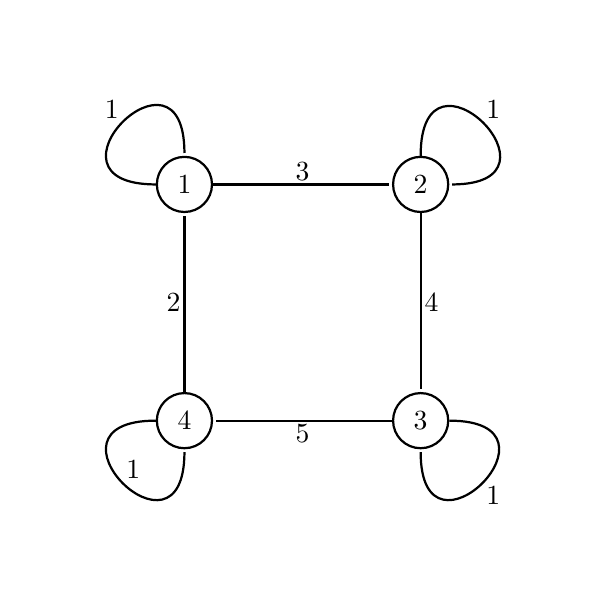
\begin{tikzpicture}[shorten >=1pt,auto,node distance=3cm,
  thick,main node/.style={circle,draw,minimum size=7mm}]

  \node[main node] (1) {1};
    \node[main node] (2) [right of=1] {2};
  \node[main node] (3) [below of=2] {3};
  \node[main node] (4) [below of=1] {4};

  \path[every node/.style={fill=white,inner sep=1pt}, every loop/.style={}]
    (1) edge[in=90,out=180, loop] node {1} (1)
        edge node {3} (2)
    (2) edge[in=0, out=90, loop] node {1} (2)
        edge node {4} (3)
    (3) edge[in=270, out=0, loop] node{1} (3)
        edge node {5} (4)
    (4) edge[in=270, out=180, loop] node{1} (4)
        edge node {2} (1)
        ;
\end{tikzpicture}
\end{center}
\begin{enumerate}[nolistsep,label=(\alph*)]
    \item Model the stochastic process \( X_n \) as a Markov chain by drawing its state transition diagram and write the corresponding one-step transition probability matrix.
    \item Calculate the stationary distribution that your token is at node \( j \), for \( j = 1, 2, 3, 4 \).
    \item Find the expected number of token moves between two consecutive visits to node 2.
\end{enumerate}
\end{problem}

\begin{solution}[Solution]
\begin{enumerate}[label=(\alph*)]
    \item We have transition diagram, 
    \begin{center}
    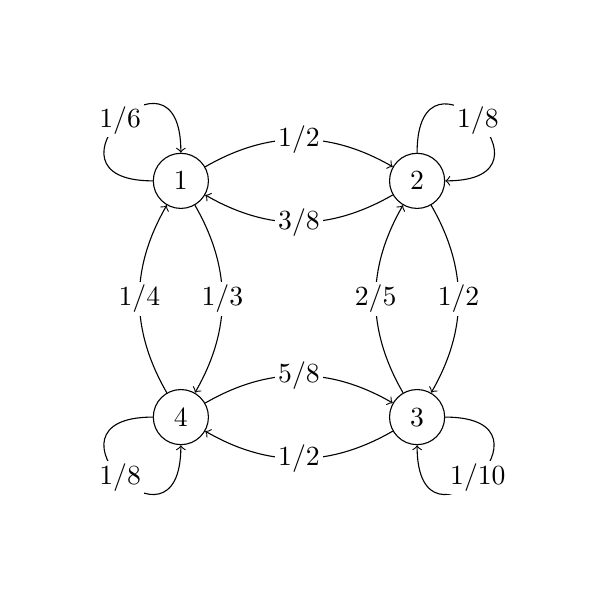
\begin{tikzpicture} 

    \draw node[circle, draw, minimum size=7mm] (1) at (0,3) {1};
    \draw node[circle, draw, minimum size=7mm] (2) at (3,3) {2};
    \draw node[circle, draw, minimum size=7mm] (3) at (3,0) {3};
    \draw node[circle, draw, minimum size=7mm] (4) at (0,0) {4};


        \path[->,every node/.style={fill=white,inner sep=1pt}, every loop/.style={->}]
    (1) edge[in=90,out=180, loop] node {1/6} (1)
        edge[bend left=30] node {1/2} (2)
        edge[bend left=30] node {1/3} (4)
    (2) edge[in=0, out=90, loop] node {1/8} (2)
        edge[bend left=30] node {1/2} (3)
        edge[bend left=30] node {3/8} (1)
    (3) edge[in=270, out=0, loop] node{1/10} (3)
        edge[bend left=30] node {1/2} (4)
        edge[bend left=30] node {2/5} (2)
    (4) edge[in=270, out=180, loop] node{1/8} (4)
        edge[bend left=30] node {1/4} (1)
        edge[bend left=30] node {5/8} (3)
        ;
    \end{tikzpicture}
    \end{center}

        The corresponding probability transition matrix \( P \) is,
        \begin{align*}
            P = \left[\begin{array}{cccc}
                1/6 & 1/2 & 0 & 1/3 \\
                3/8 & 1/8 & 1/2 & 0 \\
                0 & 2/5 & 1/10 & 1/2 \\
                1/4 & 0 & 5/8 & 1/8
            \end{array}\right]
        \end{align*} 
    \item 
        We easily compute the right eigenvector corresponding to eigenvalue \( 1 \) as,
        \begin{align*}
            \pi = \frac{1}{4}[3/4,1,5/4,1] = [3/16,1/4,5/16,1/4]
        \end{align*}
        
    \item The expected number of moves is the mean recurrence time. This chain is irreducible so by theorem we have,
        \begin{align*}
            \tau_2 = 1/\pi(2) =4
        \end{align*}
        
\end{enumerate}
\end{solution}


\begin{problem}[Practice Exam 6, Problem 2]
    Fix a probability space \( (\Omega,\cF,\PP) \) and a filtration \( \bF = (\cF_t)_{t\geq 0} \). Let \( X \) be an OU process, and \( S \) a strictly increasing L\'evy process (also known as a subordinator), whose dynamics are given by,
    \begin{align*}
        \d X_t = - X_t \d t + \sqrt{2}\d W_t, && \d S_t = \gamma \d t + \int_0^\infty z N(\d t,\d z), && S_0 = 0
    \end{align*}
    where \( W \) is a \( (\PP,\bF) \)-Brownian motion and \( N \) is a poisson random measure with associated L\'evy measure \( \nu \). Consider a Subordianted OU process \( Y \) defined as follows,
    \begin{align*}
        Y_t = X_{S_t}
    \end{align*}
    Define the two-parameter semigroup \( \cP(t,T) \) associated with the \( Y \) process,
    \begin{align*}
        \cP(t,T) f(y) := \EE[f(Y_T) | Y_t = y]
    \end{align*}
    For a fixed \( 0\leq t\leq T <\infty \), what are the eigenfunctions and associated eigenvalues of the operator \( \cP(t,T) \)?
\end{problem}

\begin{solution}[Solution]
    We first compute eigenvalues and eigenfunctions of \( \cQ(t,T) \) defined by \( \cQ(t,T)f(y) =  \EE[f(X_T)|X_t = x] \).

    We know that \( X \) has transition density,
    \begin{align*}
        \Gamma_X(t,x;T,y) = m(y) \sum_{n=0}^{\infty}H_n(x)H_n(y)e^{\lambda_n (T-t)}, && \lambda_n = n+1
    \end{align*}

    Therefore,
    \begin{align*}
        \cQ(t,T)f(y) &= \EE[f(X_T)|X_t = x] 
        = \int_\RR f(y) \Gamma_X(t,x;T,y) \d y
    \end{align*}

    Now expanding the sum,
    \begin{align*}    
        \cQ(t,T)f(y) &= \int_\RR f(y) m(y)\sum_{n=0}^\infty H_n(x)H_n(y) e^{\lambda_n (T-t)} \d y 
        \\&= \sum_{n=0}^{\infty} H_n(x)e^{\lambda_n (T-t)} \int_{\RR} f(y) H_n(y) m(y) \d y
        \\&= \sum_{n=0}^{\infty} H_n(x) e^{\lambda_n (T-t)} \ip{f,H_n}_m
    \end{align*}

    Now observe that for non-negative integer \( k \), since \( \ip{H_k,H_n} = \delta_{k,n} \),
    \begin{align*}
        \cQ(t,T) H_k(y) = \sum_{n=0}^{\infty} H_n(x) e^{\lambda_n (T-t)} \ip{H_k,H_n}_m
        = H_k(x)e^{\lambda_k (T-t)}
    \end{align*}

    Therefore \( H_k \) is an eigenvector of \( \cQ(t,T) \) with eigenvalue \( e^{\lambda_k (T-t)} \).

    Now observe,
    \begin{align*}
        \cP(t,T)f(y) &= \EE[f(Y_T) | Y_t = y]
        = \EE[f(X_{S_T})|X_{S_t}=y]
    \end{align*}

    Now, by conditional averaging,
    \begin{align*}
        \cP(t,T)f(y) = \EE[\EE[f(X_{S_T}) | S_t,S_T, X_{S_t} = y] | X_{S_t}= y]
        = \EE[\cQ(S_t,S_T)f(y) | X_{S_t} =y ]
    \end{align*}
    
    Therefore,
    \begin{align*}
        \cP(t,T)H_n(y) 
        = \EE[\cQ(S_t,S_T) H_n(y) | X_{S_t} = y]
        = \EE[e^{\lambda_n (S_T-S_t)} H_n(y) | X_{S_t} = y]
    \end{align*}
    
    Let \( \phi(s) = \EE[e^{isZ_{T-t}}] \) where \( Z_{T-t} = -i S_{T-t} \). Then, using the stationary increments property of \( S \) and the fact that \( S_0 = 0 \),
    \begin{align*}
        \cP(t,T)H_n(y) = \EE[e^{i \lambda_n S_{T-t}} H_n(y) | X_0 = y] = \phi(\lambda_n) H_n(y)
    \end{align*}

    \note{DID SOME SKETCHY SHIT HERE}
    
    



\end{solution}


\begin{problem}[Practice Exam 7, Problem 1]
\begin{enumerate}[nolistsep,label=(\alph*)]
    \item (Weather chain) The weather can be either sunny, smoggy, or rainy. The weather stays sunny for an exponentially distributed amount of time with mean 3 days and then turns smoggy. It stays smoggy for an exponentially distributed amount of time with mean 4 days and then turns rainy. Finally, it rains for an exponentially distributed amount of time with mean 1 and then it is sunny. Model the weather system as a continuous time Markov chain and compute its stationary distribution.
    \item (Barbershop) Consider a barbershop with one barber and two waiting chairs. The barber cuts hair at rate 3 customers per hour (exponentially distributed hair-cutting time). Customers arrive according to a Poisson process with rate 2 per hour. Arriving customers leave immediately if they find that the two waiting chairs are occupied. Model this system as a continuous time Markov chain and derive its stationary distribution.
\end{enumerate}
\end{problem}

\begin{solution}[Solution]
\begin{enumerate}[label=(\alph*)]
    \item Let the state space be \( \{1,2,3\} \) where 1 means sunny, 2 means smoggy, and 3 means rainy.
        By definition of the generator of the Markov process we have generator,
        \begin{align*}
            G = \left[\begin{array}{rrr}
            -1/3 & 1/3 & 0 \\
                0 & -1/4 & 1/4 \\
            1 & 0 & -1
            \end{array}\right]
        \end{align*}
        
        We can easily verify that \( \pi G = 0 \) if,
        \begin{align*}
            \pi = [3/8,1/2,1/8]
        \end{align*} 

    \item 
        Let the state space \( \{0,1,2,3\} \) denote the number of people in the queue. 
        By definition of the generator of a Markov process we have generator,
        \begin{align*}
            G= \left[\begin{array}{rrrr}
                -2 & 2 \\
                3 & -(3+2) & 2 \\
                & 3 & -(3+2) & 2 \\
                & & 3 & -3
            \end{array}\right]
        \end{align*}

        We can easily verify that \( \pi G = 0 \) if,
        \begin{align*}
            \pi = [27, 18, 12 , 8]/65
        \end{align*}     


\end{enumerate}
\end{solution}


\begin{problem}[Practice Exam 7, Problem 2]
    Fix a probability space \( (\Omega,\cF,\PP) \) and a filtration \( \bF = (\cF_t)_{0\leq t\leq T} \). Consider two processes,
    \begin{align*}
        \d X_t = \sigma_t \d W_t, && \d S_t = \sigma_t S_t \d W_t
    \end{align*}
    where \( W \) is a \( (\PP,\bF) \)-Brownian motion and the process \( \sigma = (\sigma_t)_{0\leq t\leq T} \) evolves independently of \( W \).
\begin{enumerate}[nolistsep,label=(\alph*)]
    \item Show that,
        \begin{align*}
            \EE[G(X_T-X_t)|\cF_t] = \EE[G(X_t-X_T)|\cF_t]
        \end{align*}
    \item Show that,
        \begin{align*}
            \EE[G(S_T)|\cF_t] = \EE[(S_T/S_t) G(S_t^2/S_T) | \cF_t]
        \end{align*}
        
\end{enumerate}

\end{problem}

\begin{solution}[Solution]
\begin{enumerate}[label=(\alph*)]
    \item Note that,
        \begin{align*}
            X_T - X_t = \int_t^T \sigma_t \d W_t
            , && 
            X_t - X_T = -\int_t^T \sigma_t \d W_t = \int_t^T \sigma_t \d (-W_t)
        \end{align*}
        Since \( W_t \) and \( -W_t \) are both Brownian motions distributed in the same way, then \( X_T-X_t \) and \( X_t - X_T \) are distributed in the same way. Therefore,
        \begin{align*}
            \EE[G(X_T-X_t) | \cF_t ] = \EE[G(X_t-X_T) | \cF_t]
        \end{align*}
        
    \item
        Recall that \( S_t \) has explicit representation, 
        \begin{align*}
            S_t = S_0 \exp\left(\int_0^t \left( -\frac{1}{2}\sigma_s^2 \right) \d s + \int_0^t \sigma_s\d W_s \right)
        \end{align*}

        
        Define \( Z_T = S_T/S_t \) and note that since \( S_t \) is a martingale,
        \begin{align*}
            \EE[Z_T] = \EE[\EE[Z_T | \cF_t]] = \EE[\EE[S_T/S_t | \cF_t]] = \EE[(1/S_t) \EE[S_T|\cF_t]] = \EE[S_t/S_t] = 1
        \end{align*}
        
        Therefore \( Z_T \) is a Radon--Nikod\'ym derivative process. By theorem, for \( Y \in \cF_T \) we have,
        \begin{align*}
            \tilde{\EE}[Y  |\cF_t] = \frac{1}{Z_t} \EE[Z_T Y | \cF_t] = \EE[Z_T Y | \cF_t]
        \end{align*}
        
        Note that \( Z_T \) has explicit representation,
        \begin{align*}
            Z_T = S_T/S_t = \exp \left( \int_t^T \left( -\frac{1}{2}\sigma_s^2 \right)\d s + \int_t^T \sigma_s \d W_s \right)
        \end{align*}

        Therefore, by Girsanov's theorem, \( \tilde{W}_t \) given by,
        \begin{align*}
            \d \tilde{W}_t = -\sigma_t \d t + \d W_t, && \tilde{W}_0 = 0
        \end{align*}
        is a Brownian motion under the tilde measure.
        
        Rewriting \( W_t \) in term sof \( \tilde{W}_t \) we find,
        \begin{align*}
%            S_t &= S_0 \exp \left( \int_{0}^{t} \left( -\frac{1}{2}\sigma_s^2 \right)\d s + \int_{0}^{t} \sigma_s \d W_s \right)
 %           = S_0 \exp \left( \int_{0}^{t} \frac{1}{2}\sigma_s^2  \d s + \int_0^t \sigma_s \d \tilde{W}_s \right)
  %          \\
            Z_T &= \exp \left( \int_{t}^{T} \left( -\frac{1}{2}\sigma_s^2 \right)\d s + \int_{t}^{T} \sigma_s \d W_s \right)
            = \exp \left( \int_{t}^{T} \frac{1}{2}\sigma_s^2 \d s + \int_{t}^{T} \sigma_s \d \tilde{W}_s \right)
        \end{align*}

        Now define,
        \begin{align*}
            \tilde{S}_T = S_t/Z_T &= S_t \exp \left( \int_{t}^{T} \left( -\frac{1}{2}\sigma_s^2 \right)\d s + \int_{t}^{T} \sigma_s \d (-\tilde{W}_s) \right)
        \end{align*}
       
        Since \( -\tilde{W}_t \) is a Brownian motion under the tilde measure, \( \tilde{S}_T \) is distributed the same as \( S_T \) under their respective measures. 
        Therefore,
        \begin{align*}
            \EE[(S_T/S_t) G(S_t^2/S_T) | \cF_t] 
            &= \EE[Z_T G(S_t/Z_T) | \cF_t] 
            \\&= \tilde{\EE}[ G(S_t/Z_t) | \cF_t] 
            \\&= \tilde{\EE}[G(\tilde{S}_T) | \cF_t]
            \\&= \EE[G(S_T)|\cF_t]
        \end{align*}
        
                



\end{enumerate}
\end{solution}


\begin{problem}[Practice Exam 8, Problem 1]
A bakery uses a two-step process to make chocolate cakes. The first step involves baking the cake and the second step involves frosting the cake. Baking takes an exponentially distributed amount of time with rate \( \mu_1 \) . After a cake is baked, it goes to the frosting machine. Frosting takes an exponentially distributed amount of time with rate \( \mu_2 \). The processing times at the oven and the frosting machine are independent random variables. Potential cakes arrive according to a Poisson process at rate \( \lambda \), however, a cake goes to the baking oven only if both the oven and the frosting machine are idle. If any of the two is busy, the cake simply exits the system. We wish to model this system as a continuous-time Markov chain.
\begin{enumerate}[nolistsep,label=(\alph*)]
    \item Precisely define the states of your continuous-time Markov chain (Hint: your model should have three states and note that there will never be two cakes in this system).
    \item Draw a transition diagram for your continuous-time Markov chain.
    \item Derive stationary distribution for your continuous-time Markov chain.
    \item Find the expected number of cakes in this system in steady-state.
\end{enumerate}
\end{problem}

\begin{solution}[Solution]
\begin{enumerate}[label=(\alph*)]
    \item Note that there will never be 2 cakes in the system since cakes only arrive if there are no cackes in the oven or froster.

        Then let \( S = \{\text{no cakes}, \text{cake in oven}, \text{cake in froster}\} \) be the state space.

    \item

        Our picture is a cycle,
        \begin{align*}
            \text{no cakes} &\rightarrow \text{cake in oven}
            \\
            \text{cake in oven} &\rightarrow \text{cake in froster} 
            \\
            \text{cake in froster} &\rightarrow \text{no cakes}
        \end{align*} 

        We have generator,
        \begin{align*}
            G = \left[\begin{array}{rrr}-\lambda & \lambda \\ & - \mu_1 & \mu_1 \\ \mu_2 & & -\mu_2\end{array}\right]
        \end{align*}

    \item
        Solving \( \pi G = 0 \) subject to \( \norm{\pi}_\infty = 1 \) gives,
        \begin{align*}
            \pi = \frac{1}{ \mu_1\mu_2 + \lambda(\mu_1+\mu_2)} [\mu_1\mu_2, \lambda \mu_2, \lambda \mu_2]
        \end{align*}
        
    \item The chain is irreducible so the stationary distribution above is unique. 

        The expected number of cakes in this distribution is \( 0 \cdot \pi(0) + 1 \cdot \pi(2) + 1 \cdot \pi(3) \). Expliciltly,
        \begin{align*}
            \frac{\lambda (\mu_1+\mu_2)}{\mu_1\mu_2 + \lambda(\mu_1+\mu_2)}
        \end{align*}

        As \( \lambda\to \infty \) the expected number of cakes becomes one (cakes arrive immediatley). Similarly, if \( \lambda \to 0 \), the expected number of cakes becomes 0 (cakes never arrive). 

        If \( \mu_1\to 0 \) or \( \mu_2\to 0 \), the expected number of cakes becaomes one (cakes always in oven or always in froster). 
        
        If \( \mu_1,\mu_2\to\infty \), the expected number of cakes becomes 0 (really quickly making cakes).

        Therefore, our result matches our intuition for these limiting cases.

\end{enumerate}
\end{solution}


\begin{problem}[Practice Exam 8, Problem 2]
    Fix a probability space \( (\Omega,\cF,\PP) \) and a filtration \( \bF = (\cF_t)_{0\leq t\leq T} \). Define a procecss \( X \) and stoppting time \( \tau \) as follows,
    \begin{align*}
        \d X_t = \mu \d t + \sigma \d W_t, && \tau = \inf\{t\geq 0: X_t\notin(a,b)\}
    \end{align*}
    where \( W \) is a \( (\PP,\bF) \)-Brownian motion. Define the following Laplace Transform,
    \begin{align*}
        L(x;\lambda) := \EE[e^{-\lambda \tau} | X_0 = 0), && x\in(a,b)
    \end{align*}
    Derive the PDE satisfied by \( L \) and use this to find \( L \) explicitly.
\end{problem}

\begin{solution}[Solution]

    In Theorem 9.4.1 Take \( t=0 \), \( \varphi=1 \), and \( g = 0 \). Then for \( x\in(a,b) \), \( L \) satisfies,
    \begin{align*}
        (\cA - \lambda) L = 0, && \cA = \mu \partial_ + \frac{1}{2}\sigma^2\partial_x^2
    \end{align*}
    and on the boundary,
    \begin{align*}
        L(a,\lambda) = L(b,\lambda) = 1
    \end{align*}
    

This has general form,
\begin{align*}
    L(x,\lambda) = C e^{x z_1} + D e^{x z_2}
\end{align*}
where,
\begin{align*}
    z_1 = \frac{-\mu - \sqrt{\mu^2+2\lambda \sigma^2}}{\sigma^2}
    ,&&
    z_2 = \frac{-\mu + \sqrt{\mu^2+2\lambda \sigma^2}}{\sigma^2}
\end{align*}

We solve for \( C \) and \( D \) using the boundary conditions and find,
\begin{align*}
    C = \frac{e^{a z_2} - e^{b z_2}}{e^{bz_1+az_2}-e^{az_1+bz_2}}
    ,&&
    D = \frac{e^{a z_1} - e^{b z_1}}{e^{az_1+bz_2}-e^{bz_1+az_2}}
\end{align*}



\end{solution}



